\chapter{Motor characteristics}\label{chap: B}
%
The manufacturer data-sheet contains basic characteristics of the motor as it can be seen in the \ref{table:forfor}. There are some parameters that are required for simulation purposes and are not listed in the table bellow and consequently have to be addressed. The parameters are the friction torque $T_{fric}$ which give rise to the calculation of the friction coefficient $b$, and the back $emf$ constant $k_{e}$.     
%
%\begin{figure}[H]
%	\centering
%	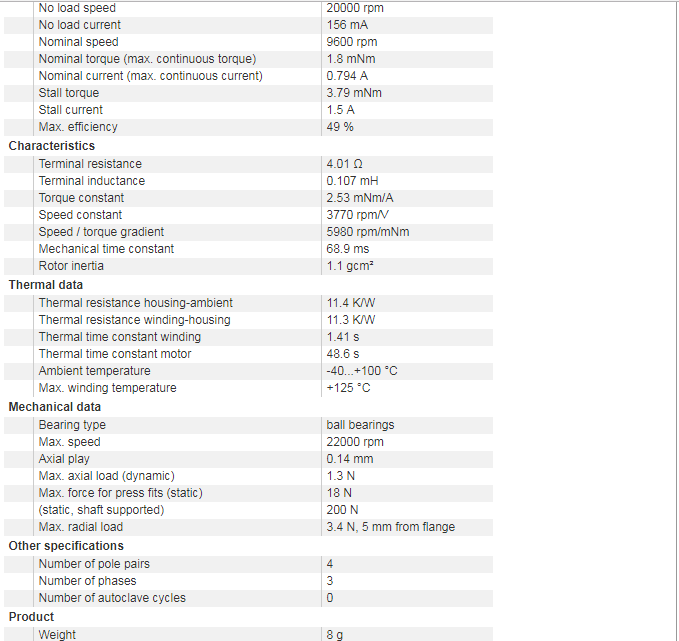
\includegraphics[width=0.7\linewidth]{figures/motorchar}
%	\caption{ Flat motor $Ø$ 13.6 mm, brushless, 1.5 Watt, sensorless with 6V nominal voltage}
%	\label{fig:323}
%\end{figure}
\begin{table}[H]
	\centering
	\begin{tabular}{|l|l|}
		\hline
		\textit{\textbf{Characteristics}}  & \textit{\textbf{Value}}                     				\\ \hline
		No load speed                      & 20000 {[}$rpm$ {]}                      					\\ \hline
		No load current                    & 156 {[}$mA${]}                             				\\ \hline
		Nominal speed                     	& 9600{[}$rpm${]}                                         	\\ \hline
		Nominal torque                     		& 1.8 [$mNm$]                                    		\\ \hline
		Nominal current                  	      & 0.794 {[}$A${]}  	
		\\ \hline
		stall torque                  	      & 3.79 {[}$mNm${]}                               			\\ \hline
		stall current                   & 1.5 {[}$A$ {]}                                     		
		 \\ \hline
		Terminal resistance  & 4.1 {[}$Ohm$ {]}                            				
		\\ \hline
		Terminal inductance     & 0.107 {[}$mH${]}                           	  				
		\\ \hline
		speed constant             & 3770 {[}$rpm/V${]}   					    \\ \hline
		Rotor inertia & 1.1 {[}$gc m^{2}${]}                               	
		 \\ \hline
		 Max speed  & 22000 {[}$rpm${]}                               	
		 \\ \hline
		 weight  & 8 {[}$g${]}                               	
		 \\ \hline
	\end{tabular}
	\caption{Flat motor $Ø$ 13.6 mm, brushless, 1.5 Watt, sensorless with 6V nominal voltage}
	\label{table:forfor}
\end{table}
Some of the torque in the mechanical part of the motors is used to overcome the friction and the rest is used in the motor shaft. An expression can be derived as
 \begin{equation*}
 T_{m} = T_{shaft} - T_{fric}
 \end{equation*}
  where $T_{m}$ is the nominal torque. Using the motor torque constant from the data sheet, $T_{fric}$ can be calculated as 
 \begin{equation*}
 T_{fric}	= k_{t}*I_{nom} - T_{m} 
 \end{equation*}    
where $I_{nom} $[A] is the nominal current. Viscous friction coefficient $b$ can now be calculated as
\begin{equation*}
	b	= \frac{T_{fric} }{\omega_{no-load}}
\end{equation*}
and $\omega_{no-load}$ is expressed in $rad/sec$. Finally, the back $emf$ constant is calculated as
\begin{equation*}
	k_{e}	= \frac{V_{nom} - I_{nom}R}{\omega_{no-load}}
\end{equation*}
where $V_{nom}$ is the nominal voltage and is equal to 6[V] and  $R$[Ohm] is the terminal resistance. 